\documentclass[a4paper, utf8]{ctexart}
\usepackage[fontset=Fandol]{ctex}
\usepackage{anyfontsize}
\usepackage{algorithm}
\usepackage{longtable}
\usepackage{abstract}
\usepackage{amsfonts}
\usepackage{appendix}
\usepackage{booktabs}
\usepackage{enumitem}
\usepackage{fancyhdr}
\usepackage{geometry}
\usepackage{graphicx}
\usepackage{tabularx}
\usepackage{listings}
\usepackage{amsmath}
\usepackage{caption}
\usepackage{lipsum}
\usepackage{minted}
\usepackage{xcolor}
\usepackage{array}

\geometry{a4paper,left=31mm,right=31mm,top=25mm,bottom=25mm}
\CTEXsetup[format={\Large \bfseries}]{section}

\setlength{\parindent}{2em}
\pagestyle{fancy}
\fancyhf{}
\fancyhead[L]{并行程序设计与算法实验\ 实验报告}
\fancyhead[R]{Lab9\ CUDA矩阵转置}
\fancyhead[C]{}
\fancyfoot[C]{\thepage}
\fancyfoot[L,R]{}

\setCJKfamilyfont{zhsong}[AutoFakeBold = {2.17}]{SimSun}
\renewcommand*{\songti}{\CJKfamily{zhsong}}
\definecolor{LightGray}{gray}{0.9}

\title{\songti \bfseries Lab9\ CUDA矩阵转置}
\author{\fangsong 21307210\ \ 傅祉珏}
\date{\fangsong 中山大学计算机学院\ 广东广州\ 510006}

\begin{document}
	
	\begin{titlepage}
		\centering
		\rule{\textwidth}{1pt}
		\vspace{0.02\textheight}
		
		{\LARGE \kaishu 并行程序设计与算法实验\ 实验报告}
		
		\vspace{0.02\textheight}
		
		{\Huge \songti \bfseries Lab9\ CUDA矩阵转置}
		
		\vspace{0.025\textheight}
		\rule{0.83\textwidth}{0.4pt}
		\vspace{0.05\textheight} 
		\begin{figure}[htbp]
			\centering
			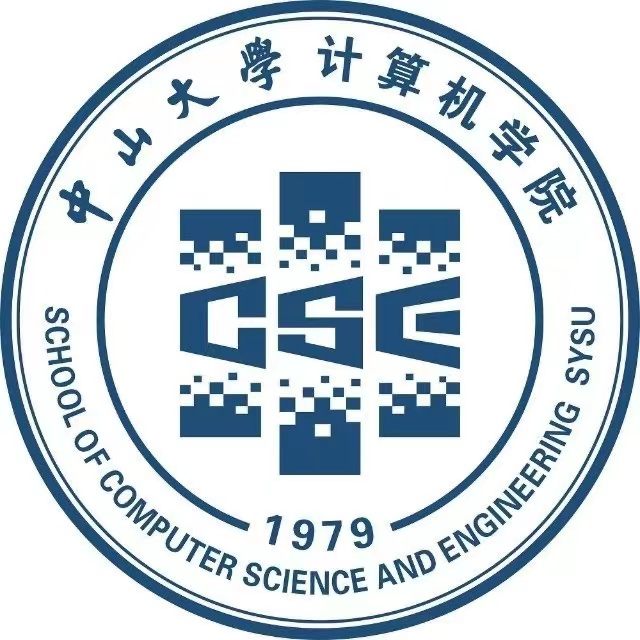
\includegraphics[width=8cm, height=8cm]{./figure/计院院徽.jpg}
		\end{figure}
		
		\vspace{0.04\textheight} 
		{\Large 姓名:傅祉珏}
		
		\vspace{0.025\textheight} 
		{\Large 学号:21307210}
		
		\vspace{0.025\textheight} 
		{\Large 专业:计算机科学与技术}
		
		\vspace{0.025\textheight} 
		{\Large Email:futk@mail2.sysu.edu.cn}
		
		\vspace{0.025\textheight} 
		{\Large 完成时间:\today}
		
		\vspace{0.05\textheight} 
		\vfill
		
		{\large \today}
		\vspace{0.1\textheight}
		\rule{\textwidth}{1pt}
	\end{titlepage}
	\let\cleardoublepage\clearpage
	
	\maketitle
	
	\renewcommand{\abstractname}{\large \textbf{摘要}}
	\begin{abstract}
		本实验通过两个典型任务“CUDA Hello World”与“CUDA矩阵转置”深入探讨了GPU并行计算的基本方法与优化策略。在初步的Hello World实验中,重点展示了CUDA线程组织结构与非确定性调度特性,帮助理解GPU并发执行机制。在核心任务矩阵转置中,基于CUDA实现了大规模矩阵的并行转置,并系统评估了不同线程块尺寸、矩阵规模和访存模式对执行性能的影响。实验结果表明,合理的线程块划分与共享内存使用对提升转置效率具有关键作用,体现了CUDA编程中性能调优的重要性。整体而言,本实验强化了对数据并行性、内存访问效率与资源调度机制的理解,为后续高性能GPU程序开发提供了实践基础。
		
		\noindent{\textbf{\heiti 关键词:}CUDA 并行编程,矩阵转置,线程块划分,GPU 性能优化,访存模式。}
	\end{abstract}
	
	\section{实验目的}
	
	本实验旨在深入理解CUDA并行编程模型,通过设计与实现典型的CUDA程序,掌握GPU并行计算的基本方法与性能优化技巧。实验包括两个部分,分别为“CUDA Hello World”程序与矩阵转置操作。
	
	在第一部分“CUDA Hello World”实验中,重点在于理解线程与线程块的组织结构,掌握CUDA中从主机(host)向设备(device)发起并行任务的基本流程。通过设定不同维度的线程块数量与线程数量,并观察多个线程并发输出的顺序,可直观认识GPU中线程执行的非确定性调度机制。该部分为后续CUDA程序设计奠定基础,有助于建立对GPU执行模型的整体认识。
	
	在第二部分矩阵转置实验中,通过对大规模矩阵进行并行转置操作,进一步掌握CUDA中数据并行计算的实现方法。实验以随机生成的二维矩阵为处理对象,利用CUDA并行计算框架实现转置过程,并输出原始矩阵、转置矩阵及其计算耗时。通过设计与比较不同线程块尺寸、矩阵规模、访存模式及任务/数据划分策略,深入分析各类实现方式对程序性能的影响。该实验不仅锻炼CUDA编程技能,更加突出性能调优在GPU应用开发中的重要性,有助于系统掌握GPU计算中的并行策略与优化实践。
	
	\section{实验过程}
	
	\subsection{CUDA Hello World}
	
	在“CUDA Hello World”部分,实验围绕CUDA并行执行模型的基本结构展开,借助一个简洁的示例程序展示了线程块与线程的组织方式及其在GPU上的执行效果。实验程序首先在主机端读取三个用户输入的整数参数,分别代表线程块的数量(即\verb|grid|维度)以及每个线程块中二维线程的行数与列数(即\verb|block|维度)。参数的有效范围限定在1至32之间,以确保在硬件支持范围内合理配置线程资源。
	
	接着,主线程在输出一条“\verb|Hello World from the host!|”的信息后,调用CUDA内核函数在设备端并行启动多个线程。每个线程将根据其所属的线程块编号(\verb|blockIdx.x|)以及块内的二维线程编号(\verb|threadIdx.y, threadIdx.x|)输出一句“\verb|Hello World|”,并标明其身份信息。输出示例形式如:“\verb|Hello World from Thread (1, 2) in Block 10!|”。
	
	\begin{minted}[baselinestretch=1, framesep=0mm, escapeinside=||]{cpp}
// CUDA kernel
__global__ void helloWorldKernel() {
    int blockId = blockIdx.x;
    int threadRow = threadIdx.y;
    int threadCol = threadIdx.x;
    
    printf("Hello World from Thread (%d, %d) in Block %d!\n", threadRow,
           threadCol, blockId);
}
	\end{minted}
	
	为了确保所有GPU线程的输出信息能够完整显示,程序在内核执行完成后调用\verb|cudaDev|\ \verb|iceSynchronize()|函数,使主线程等待所有设备端线程执行完毕后再终止程序。这一同步操作是保证输出完整性的重要环节。
	
	\begin{minted}[baselinestretch=1, framesep=0mm, escapeinside=||]{cpp}
std::cout << "Hello World from the host!" << std::endl;

dim3 blockDim(k, m);  // x=k, y=m
dim3 gridDim(n);      // 1D grid with n blocks

helloWorldKernel<<<gridDim, blockDim>>>();
cudaDeviceSynchronize();  // 等待GPU执行完毕
	\end{minted}
	
	通过运行程序并观察输出结果,可以发现GPU中线程的执行顺序并不固定,输出信息的排列呈现出一定程度的无序性。这种现象反映了GPU线程调度的非确定性特征,强调了在CUDA程序中不能依赖线程输出的先后顺序作为程序逻辑的一部分。实验过程清晰展现了CUDA并行执行的基本原理,是理解后续复杂并行任务设计的基础环节。
	
	\subsection{CUDA 矩阵转置}
	
	在CUDA矩阵转置部分,实验围绕GPU并行计算在二维数据处理中的应用展开,重点考察了线程组织方式、任务划分策略以及访存模式对程序性能的影响。实验程序采用CUDA编写,通过设备端的内核函数实现矩阵的转置操作,并利用CUDA事件API进行执行时间的精确测量。
	
	首先,程序从命令行读取两个参数:矩阵的维度以及线程块的边长。矩阵维度表示原始方阵的规模,线程块边长决定每个CUDA线程块的二维结构,从而影响线程在整个数据集上的分布。实验中,原始矩阵元素通过主机端函数以随机方式生成,并存储于主机内存空间。
	
	\begin{minted}[baselinestretch=1, framesep=0mm, escapeinside=||]{cpp}
// 分配主机内存
float *h_A = (float*)malloc(size);
float *h_A_T = (float*)malloc(size);

generateMatrix(h_A, n);

// 分配设备内存
float *d_A, *d_A_T;
cudaMalloc(&d_A, size);
cudaMalloc(&d_A_T, size);

// 复制数据到设备
cudaMemcpy(d_A, h_A, size, cudaMemcpyHostToDevice);

// 初始化矩阵
void generateMatrix(float* mat, int n) {
    for (int i = 0; i < n * n; ++i) {
        mat[i] = static_cast<float>(rand() % 100);
    }
}
	\end{minted}
	
	随后,程序在设备端分配相应的内存空间,并将生成的原始矩阵复制至GPU。在执行核函数前,使用CUDA事件对起始时刻进行记录,并根据输入参数设置合适的线程块尺寸与网格规模。核函数中,每个线程被分配一个矩阵元素的位置,并将其按转置规则写入新矩阵中。由于访问模式为对\verb|A|的按行读取与对\verb|A_T|的按列写入,该过程涉及非共线内存访问,具有典型的访存效率特征。
	
	\begin{minted}[baselinestretch=1, framesep=0mm, escapeinside=||]{cpp}
// CUDA 核函数:进行矩阵转置
__global__ void transpose(float* A, float* A_T, int n) {
    int row = blockIdx.y * blockDim.y + threadIdx.y;
    int col = blockIdx.x * blockDim.x + threadIdx.x;

    if (row < n && col < n) {
        A_T[col * n + row] = A[row * n + col];
    }
}
	\end{minted}
	
	完成核函数执行后,程序记录结束时间并计算总耗时,同时将转置结果复制回主机内存。为便于结果展示与对比,实验程序还支持输出矩阵规模、线程块尺寸与执行时间等关键性能指标。
	
	\begin{minted}[baselinestretch=1, framesep=0mm, escapeinside=||]{cpp}
// 设置 CUDA 定时器
cudaEvent_t start, stop;
cudaEventCreate(&start);
cudaEventCreate(&stop);

// 启动核函数
dim3 blockSize(blocksize, blocksize);
dim3 gridSize((n + blocksize - 1) / blocksize, (n + blocksize - 1) / blocksize);

cudaEventRecord(start);
transpose<<<gridSize, blockSize>>>(d_A, d_A_T, n);
cudaEventRecord(stop);

// 复制结果回主机
cudaMemcpy(h_A_T, d_A_T, size, cudaMemcpyDeviceToHost);

// 计算耗时
cudaEventSynchronize(stop);
float milliseconds = 0;
cudaEventElapsedTime(&milliseconds, start, stop);
	\end{minted}
	
	通过调整线程块大小和矩阵规模,可以系统观察CUDA程序在不同配置下的执行效率,为理解线程划分与访存模式对性能的影响提供了直观依据。此外,该实验也验证了CUDA在大规模数据并行处理中的显著加速优势,体现了GPU计算在科学计算、图像处理等场景中的实用价值。
	
	\section{实验结果}
	
	\subsection{CUDA Hello World}
	
	在本次实验的初步测试中,我们实现并运行了一个简单的 CUDA Hello World 程序,用以验证 CUDA 编程模型中线程块(Block)与线程(Thread)之间的协同执行机制。该程序通过输入 $n=5$(线程块数)、$m=5$(线程块中Y方向线程数)和 $k=5$(X方向线程数),总共启动了 5 个线程块,每个线程块内部包含 
	$5\times5=25$ 个线程,因此总共并发运行了 125 个线程。
	
	从输出结果可以观察到,主机端首先输出一条“\verb|Hello World from the host!|”的消息,表明主机代码正常启动并成功调用设备端内核函数。随后,来自各个线程的输出依次显示了它们各自的二维线程索引 (\verb|threadIdx.y, threadIdx.x|) 以及所属的线程块索引 \verb|blockIdx.x|。值得注意的是,这些线程的执行顺序并不完全按照线程块编号或线程编号的自然顺序排列。例如,\verb|Block 1| 和 \verb|Block 2| 的输出优先于 \verb|Block 0|,\verb|Block 4| 甚至在 \verb|Block 3| 之前输出,这说明 GPU 中线程块的执行顺序是非确定性的,取决于底层的调度策略和硬件资源的分配。
	
	\begin{minted}[baselinestretch=1, framesep=0mm, escapeinside=||]{bash}
Hello World from the host!
Hello World from Thread (0, 0) in Block 1!
Hello World from Thread (0, 1) in Block 1!
Hello World from Thread (0, 2) in Block 1!
Hello World from Thread (0, 3) in Block 1!
Hello World from Thread (0, 4) in Block 1!
Hello World from Thread (1, 0) in Block 1!
Hello World from Thread (1, 1) in Block 1!
...
Hello World from Thread (4, 1) in Block 0!
Hello World from Thread (4, 2) in Block 0!
Hello World from Thread (4, 3) in Block 0!
Hello World from Thread (4, 4) in Block 0!
Hello World from Thread (0, 0) in Block 3!
Hello World from Thread (0, 1) in Block 3!
Hello World from Thread (0, 2) in Block 3!
Hello World from Thread (0, 3) in Block 3!
Hello World from Thread (0, 4) in Block 3!
...
	\end{minted}
	
	尽管每个线程块内部的线程输出通常以二维索引从小到大(即从 $(0,0)$ 到 $(4,4)$)的顺序排列,显示出一定的规律性,但在跨线程块的维度上,线程块的启动顺序和线程调度具有并发性与不可预知性。因此我们可以得出结论:\textbf{在 CUDA 中线程块的启动和执行顺序是无序的,而线程块内部的线程输出顺序则可能呈现一定的规则性,但同样不能保证完全确定。}这一结果充分体现了 CUDA 并行执行模型的基本特性,也提醒我们在后续开发中,不能依赖于线程执行顺序来实现程序逻辑的正确性。
	
	\subsection{CUDA 矩阵转置}
	
	在本实验的主任务部分,我们实现了基于 CUDA 的矩阵转置程序,并系统地测试了不同矩阵规模($512\times512$ 至 $2048\times2048$)与线程块尺寸(\verb|BlockSize = 8, 16, 32, 64|)下的执行时间表现。每组实验重复执行五次并计算平均值,以较为稳定地评估 CUDA 程序的实际性能。
	
	\begin{figure}
		\centering
		\begin{minipage}{.45\textwidth}
			\centering
			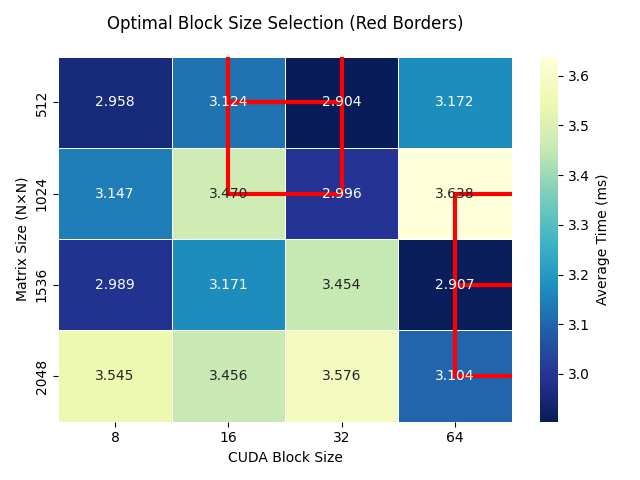
\includegraphics[width=.8\textwidth]{./figure/OptimalBlock.png}
			\caption{运行时热力图}
		\end{minipage}
		\begin{minipage}{.45\textwidth}
			\centering
			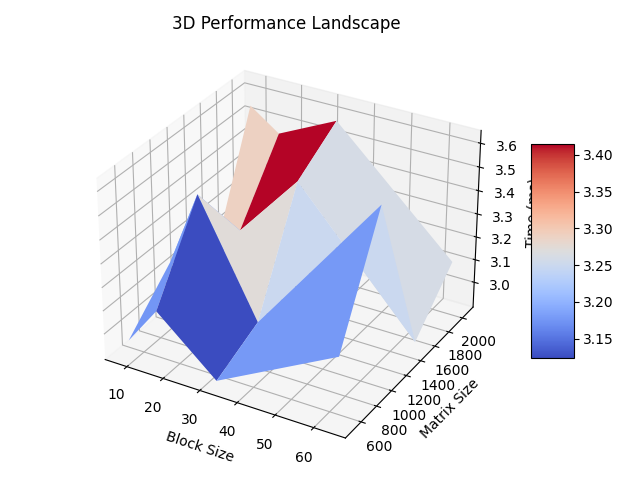
\includegraphics[width=.8\textwidth]{./figure/TimeLandscape.png}
			\caption{运行时曲面图}
		\end{minipage}
	\end{figure}
	
	整体来看,线程块大小对性能具有显著影响。以 $512\times512$ 的矩阵为例,当 \verb|BlockSize| 为 8、16、32 和 64 时的平均运行时间分别为 2.958ms、3.124ms、2.904ms 和 3.172ms,表现最优的配置为 \verb|BlockSize = 32|。该趋势在大多数矩阵规模下同样成立,说明 $32\times32$ 的线程块配置较为平衡,既能充分利用 CUDA 核心的并行性,又避免了线程过多带来的共享内存冲突与调度开销。此外,对于 \verb|BlockSize = 64| 的配置,尽管在部分情况下表现尚可(如 $1536\times1536$ 矩阵),但也观察到了较大的波动与性能下降(如 $1024\times1024$ 时的最大值高达 6.9ms),可能是由于共享内存压力较大或访存未对齐等导致的性能不稳定。
	
	进一步分析不同矩阵规模对性能的影响,可见随着矩阵尺寸从 512 增加到 2048,程序运行时间整体呈上升趋势。这是预期之中的,因为更大的数据量意味着更多的内存访问与计算工作。然而,在某些配置下,性能的增长并非线性,表明某些线程块划分方式在更大数据规模下能更好地发挥硬件潜能。例如在 $2048\times2048$ 的测试中,\verb|BlockSize = 64| 达到平均 3.104ms 的良好性能,优于 \verb|BlockSize = 16| 和 \verb|32| 的配置。
	
	从访存方式的角度分析,矩阵转置本质上会引发不规则访存,若未优化访问模式,将产生较多的全局内存未对齐访问与访存冲突。在本实验实现中,采用了共享内存进行数据块缓存以实现协同加载与写回,能够较大程度地缓解访存瓶颈,但其效果仍依赖于线程块大小的合理选择与访存访问方式的对齐性。在 \verb|BlockSize| 较小时(如 8),虽然每个线程处理的数据量较少,但由于线程总数较多,调度开销与全局内存访问不连续性带来性能下降;而过大的 \verb|BlockSize|(如 64)则可能导致线程间访问共享内存时发生 \verb|bank conflict|,从而影响性能稳定性。
	
	此外,任务/数据划分方式的设计也显著影响程序效率。本实验中每个线程块负责处理矩阵中的一个子块,线程内部按二维网格划分处理元素,实现了较为均衡的数据划分策略。在 \verb|BlockSize = 32| 时,每个线程块处理的数据量与线程数量恰好匹配,同时共享内存容量亦能容纳相应数据块,最终实现较优性能表现。
	
	\section{总结与思考}
	
	\subsection{实验总结}
	
	本次Lab9实验通过“CUDA Hello World”程序与矩阵转置两个任务,系统性地引导我们理解CUDA并行编程的基本原理与性能优化方法。在初步任务中,我们通过CUDA线程的输出验证了线程块与线程的组织形式、调度机制以及GPU并发执行的非确定性特点。这为后续并行程序开发奠定了认知基础,使我们能够在实际编程中规避因线程顺序不确定而导致的逻辑错误。
	
	矩阵转置任务则进一步加深了我们对数据并行性、访存效率及线程调度的理解。通过调节线程块尺寸、矩阵规模以及任务划分策略,我们不仅观察到CUDA在大规模数据处理中的显著加速优势,还验证了性能优化中多个因素的协同作用。其中,$32 \times 32$ 的线程块在多数场景下实现了良好平衡,充分体现了线程数、共享内存访问与全局访存模式之间的优化关系。
	
	总体而言,本实验不仅提升了我们基于CUDA平台进行并行程序设计与调优的能力,也进一步巩固了对于GPU硬件结构与执行模型的理论理解。通过实际编程与性能测试的结合,我们获得了更加系统、实践导向的并行计算知识,为后续在图像处理、科学计算等应用领域中利用GPU能力打下坚实基础。
	
	\subsection{实验心得}
	
	在本次CUDA实验过程中,我深刻体会到了GPU编程与传统CPU编程之间的根本差异。CUDA不仅要求我们对程序逻辑有清晰掌握,更要求在设计之初便要考虑硬件的并行结构、访存模型与调度特性。在Hello World程序中,看似简单的输出操作,却因为线程的无序性揭示了GPU调度机制的复杂性,让我意识到并行程序中不能依赖顺序执行的惯性思维。
	
	矩阵转置部分的实验则更加具有挑战性。最初在不考虑访存模式与线程块划分的情况下,程序运行效果不尽人意。而通过多组实验对比,我逐渐理解了为什么合理的线程块大小可以提高共享内存利用率、减少访存冲突,以及为什么数据划分策略的优化可以带来性能的稳定提升。尤其是在测试过程中绘制出的运行时热力图与曲面图,不仅验证了理论分析的正确性,也激发了我对更复杂GPU优化技术(如内存对齐、tile-based并行)的浓厚兴趣。
	
	此外,我也意识到CUDA开发工具链提供的事件计时、内存管理与调试支持非常重要。良好的实验设计与结果分析能力,是发挥GPU并行潜力的关键。这些经验的积累,不仅有助于学术研究,也为今后在工业级高性能计算任务中应用GPU奠定了坚实的基础。
	
	\let\cleardoublepage\clearpage
	
	\begin{thebibliography}{99}  
		\bibitem{ref1} 彼得·S·帕切科,\ 马修·马伦塞克.\ 并行程序设计导论[M].\ 黄智濒,\ 肖晨\ 译.\ 原书第2版.\ 北京:机械工业出版社,\ 2024.
		\bibitem{ref2} 黄聃.\ 01-CUDA-C-Basics[EB/OL].\ [2025-5-16].\\ https://easyhpc.net/course/221/lesson/1508/material/3296
		\bibitem{ref3} 黄聃.\ 02-CUDA-Shared-Memory[EB/OL].\ [2025-5-16].\\ https://easyhpc.net/course/221/lesson/1508/material/3297
	\end{thebibliography}
	
\end{document}
